% Template for PLoS
% Version 3.6 Aug 2022
%
% % % % % % % % % % % % % % % % % % % % % %
%
% -- IMPORTANT NOTE
%
% This template contains comments intended 
% to minimize problems and delays during our production 
% process. Please follow the template instructions
% whenever possible.
%
% % % % % % % % % % % % % % % % % % % % % % % 
%
% Once your paper is accepted for publication, 
% PLEASE REMOVE ALL TRACKED CHANGES in this file 
% and leave only the final text of your manuscript. 
% PLOS recommends the use of latexdiff to track changes during review, as this will help to maintain a clean tex file.
% Visit https://www.ctan.org/pkg/latexdiff?lang=en for info or contact us at latex@plos.org.
%
%
% There are no restrictions on package use within the LaTeX files except that no packages listed in the template may be deleted.
%
% Please do not include colors or graphics in the text.
%
% The manuscript LaTeX source should be contained within a single file (do not use \input, \externaldocument, or similar commands).
%
% % % % % % % % % % % % % % % % % % % % % % %
%
% -- FIGURES AND TABLES
%
% Please include tables/figure captions directly after the paragraph where they are first cited in the text.
%
% DO NOT INCLUDE GRAPHICS IN YOUR MANUSCRIPT
% - Figures should be uploaded separately from your manuscript file. 
% - Figures generated using LaTeX should be extracted and removed from the PDF before submission. 
% - Figures containing multiple panels/subfigures must be combined into one image file before submission.
% For figure citations, please use "Fig" instead of "Figure".
% See http://journals.plos.org/plosone/s/figures for PLOS figure guidelines.
%
% Tables should be cell-based and may not contain:
% - spacing/line breaks within cells to alter layout or alignment
% - do not nest tabular environments (no tabular environments within tabular environments)
% - no graphics or colored text (cell background color/shading OK)
% See http://journals.plos.org/plosone/s/tables for table guidelines.
%
% For tables that exceed the width of the text column, use the adjustwidth environment as illustrated in the example table in text below.
%
% % % % % % % % % % % % % % % % % % % % % % % %
%
% -- EQUATIONS, MATH SYMBOLS, SUBSCRIPTS, AND SUPERSCRIPTS
%
% IMPORTANT
% Below are a few tips to help format your equations and other special characters according to our specifications. For more tips to help reduce the possibility of formatting errors during conversion, please see our LaTeX guidelines at http://journals.plos.org/plosone/s/latex
%
% For inline equations, please be sure to include all portions of an equation in the math environment.  For example, x$^2$ is incorrect; this should be formatted as $x^2$ (or $\mathrm{x}^2$ if the romanized font is desired).
%
% Do not include text that is not math in the math environment. For example, CO2 should be written as CO\textsubscript{2} instead of CO$_2$.
%
% Please add line breaks to long display equations when possible in order to fit size of the column. 
%
% For inline equations, please do not include punctuation (commas, etc) within the math environment unless this is part of the equation.
%
% When adding superscript or subscripts outside of brackets/braces, please group using {}.  For example, change "[U(D,E,\gamma)]^2" to "{[U(D,E,\gamma)]}^2". 
%
% Do not use \cal for caligraphic font.  Instead, use \mathcal{}
%
% % % % % % % % % % % % % % % % % % % % % % % % 
%
% Please contact latex@plos.org with any questions.
%
% % % % % % % % % % % % % % % % % % % % % % % %

\documentclass[10pt,letterpaper]{article}
%\documentclass[10pt]{article}
%\usepackage[top=0.85in,left=2.75in,footskip=0.75in]{geometry}

\usepackage[paper=a4paper,
  inner=2.5cm,
  outer=3.8cm,
  bindingoffset=.5cm,
  top=1.5cm,
  bottom=1.5cm]{geometry}


% amsmath and amssymb packages, useful for mathematical formulas and symbols
\usepackage{amsmath,amssymb}
\usepackage{physics}
\newcommand{\pdvn}[3]{\frac{\partial^{#1} {#2}}{\partial {#3}^{#1}}}
\newcommand{\Underbrace}[2]{{\underbrace{#2}_{#1}}}

% Use adjustwidth environment to exceed column width (see example table in text)
\usepackage{changepage}

% textcomp package and marvosym package for additional characters
\usepackage{textcomp,marvosym}

% cite package, to clean up citations in the main text. Do not remove.
% \usepackage{cite}

% Use nameref to cite supporting information files (see Supporting Information section for more info)
\usepackage{nameref,hyperref}

% line numbers
\usepackage[right]{lineno}

% ligatures disabled
\usepackage[nopatch=eqnum]{microtype}
\DisableLigatures[f]{encoding = *, family = * }

% color can be used to apply background shading to table cells only
\usepackage[table]{xcolor}

% array package and thick rules for tables
\usepackage{array}

% create "+" rule type for thick vertical lines
\newcolumntype{+}{!{\vrule width 2pt}}

% create \thickcline for thick horizontal lines of variable length
\newlength\savedwidth
\newcommand\thickcline[1]{%
  \noalign{\global\savedwidth\arrayrulewidth\global\arrayrulewidth 2pt}%
  \cline{#1}%
  \noalign{\vskip\arrayrulewidth}%
  \noalign{\global\arrayrulewidth\savedwidth}%
}


% \thickhline command for thick horizontal lines that span the table
\newcommand\thickhline{\noalign{\global\savedwidth\arrayrulewidth\global\arrayrulewidth 2pt}%
\hline
\noalign{\global\arrayrulewidth\savedwidth}}


% Remove comment for double spacing
\usepackage{setspace} 
\doublespacing

% Text layout
\raggedright
\setlength{\parindent}{0.5cm}
\textwidth 5.25in
\textheight 8.75in

% Bold the 'Figure #' in the caption and separate it from the title/caption with a period
% Captions will be left justified
\usepackage[aboveskip=1pt,labelfont=bf,labelsep=period,justification=raggedright,singlelinecheck=off]{caption}
\renewcommand{\figurename}{Fig}
  
% Use the PLoS provided BiBTeX style
% \bibliographystyle{plos2015}
% Remove brackets from numbering in List of References

\makeatletter
\renewcommand{\@biblabel}[1]{\quad#1.}
\makeatother




% Header and Footer with logo

\usepackage{lastpage,fancyhdr,graphicx}
\usepackage{epstopdf}
\usepackage[bibstyle=numeric,style=authoryear-icomp,maxbibnames=10,maxcitenames=2,uniquelist=false, backend=bibtex,url=false, sorting=none]{biblatex}
\usepackage{float}



\addbibresource{manual.bib}
\AtEveryBibitem{\clearfield{note}}



%\addbibresource{Mendeley.bib}
%\addbibresource{manual.bib}
%\bibliography{references}
%\pagestyle{myheadings}
\pagestyle{fancy}
\fancyhf{}
%\setlength{\headheight}{27.023pt}
%\lhead{\includegraphics[width=2.0in]{PLOS-submission.eps}}
\rfoot{\thepage/\pageref{LastPage}}
\renewcommand{\headrulewidth}{0pt}
\renewcommand{\footrule}{\hrule height 2pt \vspace{2mm}}
\fancyheadoffset[L]{2.25in}
\fancyfootoffset[L]{2.25in}
\lfoot{\today}

%% Include all macros below

\newcommand{\lorem}{{\bf LOREM}}
\newcommand{\ipsum}{{\bf IPSUM}}

%% END MACROS SECTION

\setlength{\parskip}{\baselineskip}%
\setlength{\parindent}{0pt}%
\begin{document}
\vspace*{0.2in}

% Title must be 250 characters or less.
\begin{flushleft}
{\Large
\textbf\newline{Effects of multistability, absorbing boundaries and growth on Turing pattern formation} % Please use "sentence case" for title and headings (capitalize only the first word in a title (or heading), the first word in a subtitle (or subheading), and any proper nouns).
}
\newline
% Insert author names, affiliations and corresponding author email (do not include titles, positions, or degrees).
\\
Martina Oliver Huidobro \textsuperscript{1},
Robert G. Endres \textsuperscript{1}


\bigskip
\textbf{1} Department of Life Sciences and Centre for Integrative Systems Biology and Bioinformatics, Imperial College, London, United Kingdom
\\
\bigskip

% Insert additional author notes using the symbols described below. Insert symbol callouts after author names as necessary.
% 
% Remove or comment out the author notes below if they aren't used.
%
% Primary Equal Contribution Note
%\Yinyang These authors contributed equally to this work.

% Additional Equal Contribution Note
% Also use this double-dagger symbol for special authorship notes, such as senior authorship.
%\ddag These authors also contributed equally to this work.

% Current address notes
%\textcurrency Current Address: Life Sciences Department, Imperial College London, London, United Kingdom% change symbol to "\textcurrency a" if more than one current address note
% \textcurrency b Insert second current address 
% \textcurrency c Insert third current address

% Deceased author note
%\dag Deceased

% Group/Consortium Author Note
%\textpilcrow Membership list can be found in the Acknowledgments section.

% Use the asterisk to denote corresponding authorship and provide email address in note below.
* correspondingauthor@institute.edu

\end{flushleft}
% Please keep the abstract below 300 words

\section*{Abstract}
Turing patterns are a fundamental concept in developmental biology, describing how homogeneous tissues develop into self-organized spatial patterns. However, the classical Turing mechanism, which relies on linear stability analysis, often fails to capture the complexities of real biological systems, such as multistability, non-linearities, growth, and boundary conditions. Here, we explore the impact of these factors on Turing pattern formation, contrasting linear stability analysis with numerical simulations based on a simple reaction-diffusion model, motivated by synthetic gene regulatory pathways. We demonstrate how non-linearities introduce multistability, leading to unexpected pattern outcomes not predicted by traditional Turing theory. Additionally, the study examines how growth and realistic boundary conditions influence pattern robustness, revealing that different growth regimes and boundary conditions can either disrupt or stabilize pattern formation. Our findings are critical for understanding pattern formation in both natural and synthetic biological systems, providing insights into engineering robust patterns for applications in synthetic biology.


% Please keep the Author Summary between 150 and 200 words
% Use first person. PLOS ONE authors please skip this step. 
% Author Summary not valid for PLOS ONE submissions.   
\section*{Author summary}
During development, tissues self-organise to go from a single cell to an structured organism. In this process, simple chemical reactions lead to the emergence of the intricate designs we see in nature, like the stripes on a zebra or the labyrinths on a brain cortex. Although multiple theories have been proposed to model this phenomenon, one of the most simple and popular ones was introduced in the 50s by the mathematician Alan Turing. However, his theory oversimplifies the biological conditions and ignores properties such as non-linearities, boundary effects or growth in the tissue. In this work, we used a combination of mathematical models and computer simulations to investigate how these real-world factors influence pattern formation. Our findings show that when we account for non-linear behaviours, growth, and boundary effects, the patterns that emerge can be very different from what the Turing theory would predict. This work helps us better understand the laws behind pattern formation and could have practical applications in tissue engineering for medical or environmental applications. 

\linenumbers
%\textcite{weinberg,glashow,companion}
%\printbibliography
% Use "Eq" instead of "Equation" for equation citations.
\section{Introduction}

How biology produces robust patterns in space and time is still largely an open question~\parencite{scholes2017three}.
In 1952, Alan Turing proposed a mechanism referred to as Turing patterns or diffusion-driven instabilities, which explains how a homogeneous tissue results in self-organized spatial repetitive patterns of the network’s molecules ~\parencite{Turing1952, Gierer1972}.
However, this proposed mechanism is far from real biological complexity, and suffers from fine tuning, meaning only a small subset of constrained parameters can generate these spatial patterns.
Additionally, the diffusion-driven instability is based on linear stability analysis theory meaning natural relevant phenomena such as multistability, growth, exotic boundary conditions and non-linearities are often not addressed.
A way forward to understanding the relationship between theoretical Turing patterns and real biological patterns is to engineer these reaction-diffusion networks in biofilms using synthetic biology ~\parencite{Sekine2018, Karig2018}.
This would allow us to better understand the role of Turing patterns in biological pattern formation, as well as to engineer synthetic patterns for industrial applications~\parencite{cao2017programmable, tan2018polyamide,din2020interfacing}.
This approach was recently extended and implemented in~\cite{Oliver2023} where a Turing gene circuit was introduced in growing \textit{E.coli} colonies producing periodic spatial patterns (see Fig.~\ref{fig1}A for an example).

A realistic mathematical description of such a biological system has non-linearities, multistability, growth and boundary conditions which are not easily captured with linear stability analysis. The latter technique only describes the onset of pattern formation, not the final pattern.
Several studies have explored how these phenomena affect Turing pattern formation including non-linearities~\parencite{ermentrout1991stripes}, multistability~\parencite{Krause2023}, boundaries~\parencite{Arcuri1986,Maini1993, Maini1997,Krause2020, Krause2021, Woolley2022} and growth~\parencite{gaffney2010, Klika2017, Krause2019}.
However, these studies are often based on idealised domains, certain types of popular or convenient boundary conditions, and artificial growth assumptions.
Additionally, often they do not provide statistics of how Turing patterns become more or less robust to the fine-tuning problem when introducing these phenomena by conducting high-throughput parameter scans.
Therefore, a high-throughout numerical study is needed to understand how all these natural phenomena affect Turing pattern formation, in particular in a synthetic system such as the one in~\cite{Oliver2023}.

In this paper, we combine linear stability analysis and numerics, to study a simple Turing  reaction-diffusion network with non-linearities which leads to multistability.
Our analysis goes beyond classical Turing patterns as we also consider other types of instabilities such as Hopf and Turing-Hopf and how these can generate periodic stationary or non-stationary patterns.
We find that switching of steady states in multistable system can generate unexpected outcomes not predicted by linear stability analysis.
Additionally, growth and realistic boundary conditions are added to understand how patterning occurs in microbial colonies with synthetic Turing gene circuits (see Fig.~\ref{fig1}B-C).
We find that different boundaries and growth regimes can break or form patterns, therefore adding or removing robustness to pattern formation.
Studying how all these biological phenomena affect patterning is extremely important not only in the context of engineering patterns in synthetic biology, but also to understand how robust patterns occur in developmental biology where large gene-regulatory networks commonly exhibit non-linearities and multistability and where tissues are growing while in contact with an external environments.


% Place figure captions after the first paragraph in which they are cited.
\begin{figure}[H]
    \includegraphics[width=1\textwidth]{figures/biological_example}

    \caption{{\bf Synthetic Turing patterns from experiments and theory.}
        \textbf{(A)} Snapshot of a bacterial colony with synthetic 6-node Turing gene circuit producing periodic spatial patterns in two-dimensions (scale bar ....) (\cite{Oliver2023}). Cross section of the colony for quantifying the periodic pattern in one dimension (1D) shown by a white line. \textbf{(B)} Final snapshot of the 1D numerical solution from C. The $Y$ axis is concentration (nM) of $U$ (left, blue) and $V$ (right, red) while the $X$ axis is space (mm). \textbf{(C)} Numerical solution with absorbing boundary conditions generates a periodic pattern, plotted as a timeseries of molecule $U$. The $Y$ axis is time (h), $X$ axis is space (mm) and concentration is shown by color with blue being high concentration and red being low concentration. }
    %TODO figure caption
    \label{fig1}
\end{figure}
 
\section{Results}
To study the effects of multistability, non-linearities, boundary conditions, and growth, we use a simple reaction-diffusion model which consists of a 2-node Turing topology system with non-linear Hill-functions to represent gene activation and inhition.
The activator $A$ activates itself and $I$, while the inhibitor $I$ inhibits the activator $A$ (see Fig. 1...).


\begin{subequations}
    \begin{equation}
        \pdv{[A]}{t}=b_{A}+V_{A} \cdot\frac{1}{1+\left(\frac{K{A}}{[A]}\right)^{n_{A}}}\cdot\frac{1}{1+\left(\frac{[I]}{K_{I}}\right)^{n_{I}}}-\mu_{A}\cdot[A] + D_{A}\nabla^2 [A]
    \end{equation}

    \begin{equation}
        \pdv{[I]}{t}=b_{I}+V_{I} \cdot\frac{1}{1+\left(\frac{K{A}}{[A]}\right)^{n_{A}}}-\mu_{I}\cdot[I] +
        D_{I}\nabla^2 [I]
    \end{equation}

    \label{eq:turinghill}
\end{subequations}

[Now explain the terms and parameters in detail (one could also experiment with underbrackets for last equation to highlight synthesis, degradation, and diffusion). General Laplacian could be defined as d/dx (or short d_x) here too, to signal that it is 1D. For a math audience, one now would also need to specify the domain and the boundary conditions.]

\subsection{Multistability}
In this section, we demonstrate how linear stability analysis is not sufficient or necessary to predict Turing patterns (TPs) in multi-stable systems.
In particular, we study in detail the dynamical behaviour of multi-stable systems during pattern formation, which will lead to the creation or breaking of the pattern.
The motivation behind this arises from the high degree of multistability exhibited by biological systems, where cell-fate decisions have to be taken within this landscape ~\parencite{huang2000shape, moris2016transition}.
Multistability is especially common in systems with non-linearities and feedback loops, as the ones in biology or in our models~\parencite{pham2020complexity, leite2009multistability}.

Using the two-node non-linear Turing topology (Eq.~\ref{eq:turinghill}), multi-stable solutions were identified and studied to understand how the patterning dynamics are affected in the presents of multiple steady-state solutions.
First, linear stability analysis was carried out, as explained in \ref{lsa}, on particular parameter sets to find multiple steady states with different stability nature, e.g.~stable, unstable, Turing I, Turing I-Hopf, Hopf. Here, Turing I etc refers to.....
Second, numerical simulations were computed using the Crank-Nicholson algorithm, where the initial condition is a random uniform distribution around a particular steady state.
Different pattern outcomes result depending on the location in the phase diagram the initial condition is.
Following the classical hypothesis used in the Turing literature, we expected stable and unstable systems to not produce patterns and equations fulfilling the Turing conditions to produce patterns.
Here, we present various examples of how this hypothesis can break in the presents of multistability.

Fig.~\ref{fig:multistability1} shows a case where diffusion-driven instability conditions are not required for Turing pattern formation.
The unstable state, having a dispersion relation with a peak below zero (Fig.~\ref{fig:multistability1}C), managed to get into a Turing pattern regime as it is attracted by the neighbouring Turing steady state.
It therefore produces a stationary pattern (Fig.~\ref{fig:multistability1}B), even though its dispersion relation does not predict so.
This trajectory is depicted in the phase diagram (Fig.~\ref{fig:multistability1}A) which shows the steady states along with the vector field to understand the potential trajectories of the system.
The phase diagram does not fully capture the dynamics as it describes the system without diffusion, while the dispersion relation and the numerical solution do consider diffusion.

\begin{figure}[H]
    \includegraphics[width=1\textwidth]{figures/multistability1}

    \caption{\textbf{Stationary Patterns in multistability.} \textbf{(A)} Phase diagram without diffusion illustrating three distinct steady states where the derivative is zero: stable, unstable, and stable (Turing). These steady states are represented within a parameter space defined by two axes: concentrations of A and I. The vector field, indicated by light green arrows, shows the direction of the derivatives of the system at various points in the parameter space. A hand-drawn trajectory is also shown (dark green arrow), demonstrating how the unstable state may evolve into the Turing state. \textbf{(B)} Dispersion relation showing each type of state. \textbf{(C)} Numerical solutions of the three steady states with diffusion, where the unstable state unexpectedly produces a Turing-like stationary pattern. }
    \label{fig:multistability1} % A label for referencing this figure later in the document
\end{figure}
%TODO make font smaller in figure


Then, we present a case where LSA incorrectly predicts stationary pattern formation.
Fig.~\ref{fig:multistability2} shows an ephemeral or transient pattern that occurs in the unstable and Turing regimes.
The TP initially develops in the vicinity of the Turing steady state.
As the spatial heterogeneity is amplified and settles, it gets attracted by the stable steady state leading to the disruption of the pattern.
This type of transient pattern behaviour has also been recently reported in~\cite{Krause2023}.

\begin{figure}[H]
        \includegraphics[width=1\textwidth]{figures/multistability2} % The name of your image file; assumes it is in the same directory as your .tex file
    \caption{\textbf{Ephemeral patterns in multistability.} \textbf{(A)} Phase diagram without diffusion illustrating three distinct steady states where the derivative is zero. The hand-drawn trajectory (dark green arrow) shows an unstable state evolving into a stable (Turing), and a stable (Turing) evolving into a stable. \textbf{(B)} Dispersion relation showing each type of state. \textbf{(C)} Numerical solutions of three steady states with diffusion. Unstable and Turing produce temporary periodic stationary patterns, that then disappear and become spatially homogeneous solutions.}
    \label{fig:multistability2} % A label for referencing this figure later in the document
\end{figure}

Other interesting examples can be found, for example, where an unstable state is surrounded by two Turing states, this unstable state will robustly lead to a Turing pattern (Fig.~\ref{sup_fig4}A).
Additionally, in some cases, the unstable system settles into Turing, but the Turing system gets pulled by the stable attractor (Fig.~\ref{sup_fig4}B). Additionally, some systems even exhibit three solutions which are homogeneous in time and space (Fig.~\ref{sup_fig4}C).
In this case, it would be worth investigating earlier time points with more resolution, as a pattern might appear then.
Interesting interactions similarly occur with multistability involving Turing I-Hopf solutions which will be mentioned in the following sections (Fig.~\ref{sup_fig4}D).



\subsection{Analytical to numerical: Other types of dispersion relations, and other types of patterns} \label{nogrowth}
Multi-stable systems are not the only case where the classical Turing instability theory fails to predict pattern formation.
Other types of dispersion relations beyond classical Turing instabilities can produce stationary patterns and non-stationary regular patterns that might be of interest in developmental biology.

High-throughput studies like~\cite{Scholes2019, Zheng2016, Marcon} only consider Turing I as patterning and the rest is discarded.
Here we explore beyond Turing I and stationary patterns to give a more complete view of the relationship between linear stability and spatio-temporal patterns.
By classifying dispersion relation types and pattern types, we document what type of dispersion relations in mono-stable systems can be linked to what type of patterns, to gain insights into predicting pattern formation from linear stability analysis.

All types of dispersion relations in our parameter space were classified into 5 types:
Stable dispersion relations (Fig~\ref{fig:dispersions}A) have all eigenvalues $\sigma$ below zero for any wavenumber $k_{n}$.
Unstable dispersion relations (Fig~\ref{fig:dispersions}C) have a positive eigenvalue at $k_{0}=0$ which eventually drops below zero as diffusion is introduced (i.e. $k_{n}>0$).
Hopf-type dispersion relations, as with any unstable dispersion relation, shows an instability without diffusion ($\sigma>0$ for $k_{0}=0$) which eventually drops below zero for positive wavenumber. However, in the case of the Hopf-type dispersion relation, when the eigenvalues cross the zero line, there is a pair of complex conjugate eigenvalues (Fig~\ref{fig:dispersions}D).
A Hopf-like dispersion relation is different to a Hopf bifurcation: a bifurcation displays a shift in stability as a model parameter changes, while the Hopf-like dispersion is a change in stability as a function of the wavenumber $k_{n}$.
%In this case, the bifurcation parameter would be $k$, making the system go from unstable to stable by changing this parameter.
Turing I dispersion relations, as previously mentioned, are stable without diffusion, have an instability for a positive wavenumber, and finally become stable again for very large wavenumbers (Fig~\ref{fig:dispersions}B).
Turing I-Hopf dispersion relations, are a combination of Turing I and Hopf-type dispersion relations. As the Hopf-type dispersion, they are unstable without diffusion. Then, as $k_{n}$ is increased, the system becomes stable with a pair of complex conjugates as the eigenvalues cross the zero line.
Finally, a Turing I-type behaviour arises getting a peak above zero and decaying again for large wavenumbers (Fig~\ref{fig:dispersions}E).

Other types of dispersion relation exist which are not displayed here such as Turing II, where the eigenvalues do not become stable again for very large wavenumbers.
Therefore, this system displays an instability at very large wavenumbers which results in infinitesimally small wavelength patterns.
These are considered to produce homogeneous solutions, except in the case of space discretization where they can produce small wavelength patterns~\parencite{Wang2022}.
However, Turing II solutions are not possible in systems such as this one where all nodes are diffusing.
This is because for $k_n \rightarrow \inf$, all eigenvalues $\sigma$ must be negative (see Eq.~\ref{jacobian_diffusion}).

As with the classification of the dispersion relations, we classify the patterns produced numerically into homogeneous, temporal oscillator, non-stationary pattern and stationary pattern (see \ref{numerical_classification1}.
By classifying both LSA and numerical outputs, we can generate a new confusion matrix with information about other types of dispersion relations and other types of spatio-temporal patterns (Fig~\ref{fig:dispersions}F).

This confusion matrix shows how not only systems with a Turing I dispersion relations can generate a stationary spatial pattern. Unstable, Hopf and Turing I Hopf can produce such results too. Additionally, interesting behaviours can arise such as temporal oscillators and non-stationary patterns.

\begin{figure}[H]
    \includegraphics[width=1\textwidth]{figures/dispersion} % The name of your image file; assumes it is in the same directory as your .tex file
    \caption{\textbf{Relationship between dispersion relation and numerical solutions} \textbf{(A-E)} Examples of a dispersion relation (left) and a resulting numerical solution (right) for Stable, Turing I, Unstable, Hopf, Turing I Hopf. \textbf{(F)} Confusion matrix linking LSA output (rows) and numerical pattern outcome (columns). Numbers show the percentage of solutions across the LSA output rows.}
    \label{fig:dispersions} % A label for referencing this figure later in the document
\end{figure}


\section{Introducing biological features: Absorbing boundaries and growth}
As shown above, both multistability effects and numerical solutions can break the hypothesis that only classical Turing I systems can produce stationary periodic patterns.
Here, we look deeper into how other aspects linking the theory closer to the biological reality can also break this hypothesis.
In particular, we will look at how adding an absorbing boundary condition and growth to a reaction-diffusion system might induce or break patterning.
This particular direction was inspired by experiments described in~\parencite{Oliver2023}, where growing bacterial colonies in agar are used as a platform to engineer Turing patterns using synthetic gene circuits.

The parameter space was explored using simulations and classifying these simulations with (1) no-growth and reflective boundaries, (2) no-growth and absorbing boundaries and finally (3) growth and absorbing boundaries. This way we can understand separately the effects of absorbing boundaries and growth in a synthetic system such as~\parencite{Oliver2023}
Again, all these parameter sets have only a single steady state to ensure patterning effects are due to boundaries and growth and not due to multistability.

When absorbing boundaries or growth are added, periodic patterns might get created, disrupted or remain the same. The Sankey diagram in Fig~\ref{fig:boundariesgrowth}A shows how this system can transition when absorbing boundaries and growth are introduced.
As explained in the methods section below (see~\ref{classification}), the classification previously used cannot be used for absorbing boundary conditions as these prevent the pattern from being completely homogeneous or stationary.  %TODO ref classification. %TODO add letter to image
Therefore, a different type of classification has to be used for reflective and absorbing boundary conditions. For reflective boundary conditions we classify patterns into (1) Homogeneous, (2) Temporal Oscillators, (3) Non-stationary patterns and (4) Stationary patterns (see~\ref{numerical_classification1}). For absorbing boundary conditions we classify patterns into (1) homogeneous, (2) boundary effect, (3) weak pattern, (4) intermediate pattern and (5) strong pattern (see~\ref{numerical_classification2})
Although the classification outputs cannot be directly compared, this confusion matrix is useful to identify interesting cases:
If absorbing boundary conditions had no effect, we would expect homogeneous and temporal oscillator categories in the y-axis to become no pattern, homogeneous or boundary effect.
Additionally, we would expect stationary patterns to become strong patterns.
This is commonly the case as seen by the thicker lines in~\ref{fig:boundariesgrowth}A, which shows boundaries do not often affect the pattern.
However, some exceptions are present which are further studied in Fig~\ref{fig:boundariesgrowth}B.

In particular, we observe systems where an absorbing boundary condition make a homogeneous solution become a non-stationary pattern. Additionally, absorbing boundary conditions can turn a temporal oscillator into a stationary pattern. Finally, by adding growth, a non-stationary pattern can be stabilised into a growing stationary pattern.
\begin{figure}[H]
    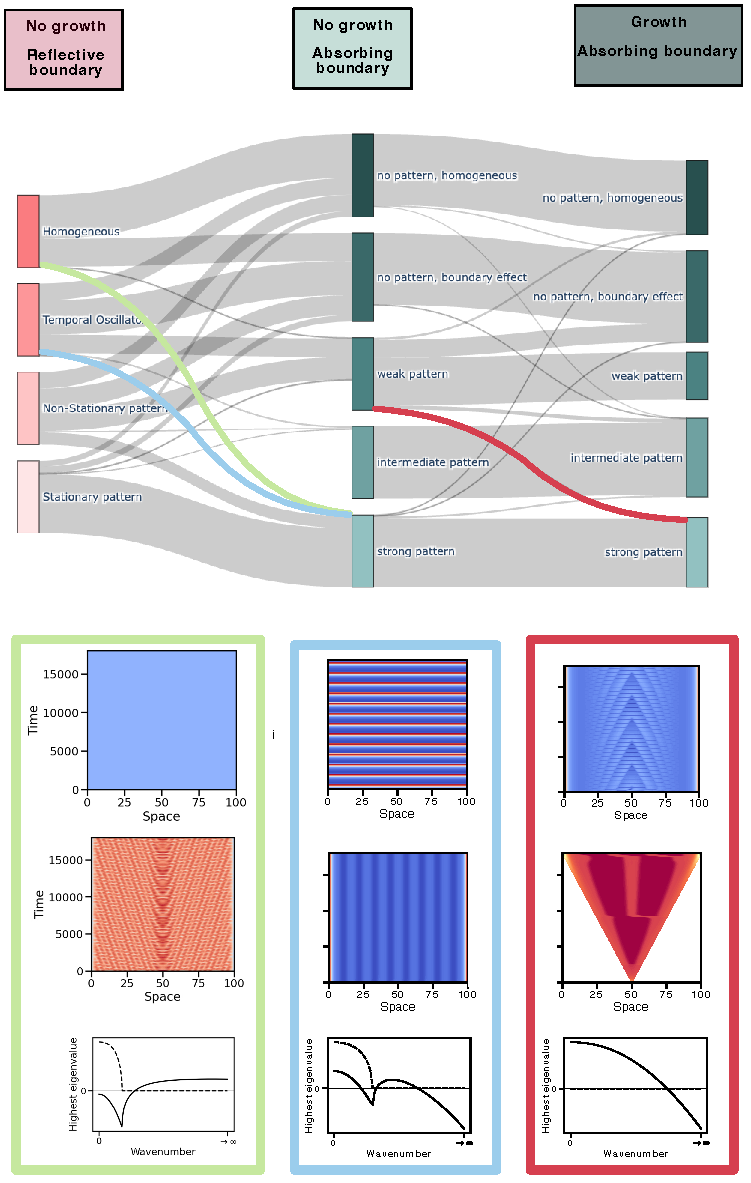
\includegraphics[width=1\textwidth]{figures/boundaries_growth} % The name of your image file; assumes it is in the same directory as your .tex file
    \caption{a}
    \label{fig:boundariesgrowth} % A label for referencing this figure later in the document
\end{figure}
\section{Discussion}
%TODO redo with chatgpt to shorten and reduce plagiarism.

%TODO check present or past tense
In this study, we utilized numerical methods to investigate how reaction-diffusion circuits can generate spatio-temporal patterns beyond the scope of linear stability analysis predictions.
The discrepancies between these LSA and numerical predictions can be attributed to non-linearities, multistability, varying boundary conditions, or growth.

Most current robustness studies primarily focus on Turing I instabilities ~\parencite{Scholes2019, Zheng2016, Marcon}.
However, we demonstrate that numerical methods for robustness searches can uncover a wider variety of relevant spatio-temporal solutions.
For example, systems exhibiting unstable, Hopf or Turing I-Hopf dispersion relations can also produce Turing-like stationary periodic patterns~\ref{fig:dispersions}F.
Therefore, systems with such dispersion relations should not be disregarded when studying pattern formation.
Although considering these systems might slightly improve robustness, it does not fully explain the difference between the robust mechanisms of nature and the non-robust Turing patterns.
Additionally, some systems with a Hopf dispersion relation produce noteworthy non-stationary periodic patterns.
These non-stationary patterns could be highly valuable in developmental and synthetic biology because gene expression arrest could transform them into periodic stationary patterns.
Furthermore, these non-stationary patterns might act as a periodic pre-pattern for initial symmetry breaking.
Overall, when considering symmetry-breaking events and periodicity in developmental biology, it is important to look beyond classical Turing dispersion relations and consider Hopf, Turing I-Hopf, and simple unstable systems that might also explain periodic patterning in biology.
Therefore, in the context of symmetry-breaking events and periodicity in developmental biology, it is crucial to consider beyond traditional Turing dispersion relations and include Hopf, Turing I-Hopf, and simple unstable systems as potential explanations for biological periodic patterning.

We have also explored the influence of multistability on Turing systems.
We describe the mechanism by which unstable systems can acquire Turing pattern dynamics through multistability and how Turing states can lose their patterning.

Moreover, we introduce ephemeral patterns, which are transient patterns occurring as the system transitions from Turing to stable states.
T These ephemeral patterns could be significant for developmental biology because they might temporarily activate the necessary genes to produce a permanent phenotype.
For instance, digit formation requires periodic patterns only at specific times when growth hormone is produced to generate fingers ~\parencite{raspopovic2014digit}.
Understanding how interactions between different steady states influence pattern formation is essential, as multistability is widespread and plays a critical role in biological systems~\parencite{laurent1999multistability}.

 Absorbing boundaries and growth, which were studied following the experimental setup in ~\parencite{Oliver2023}, also determine the outcome of spatio-temporal patterns.
Introducing absorbing boundary conditions generally results in more interpretable outcomes compared to growth, as the same classification system is used.
A significant proportion of cases fall into the top diagonal of the confusion matrix (Fig.~\ref{sup_fig5}A), suggesting that absorbing boundary conditions might enhance patterning robustness.
Specifically, absorbing boundaries can induce spatial patterning by creating non-stationary or stationary periodic patterns from spatially homogeneous patterns (Fig.~\ref{fig:boundariesgrowth}B,C).
However, adding absorbing boundaries can also disrupt spatial patterns, as shown in the Sankey diagram (Fig.~\ref{fig:boundariesgrowth}A).
This underscores the importance of looking beyond linear stability analysis and considering different boundary conditions when studying spatio-temporal patterning.

As opposed to adding absorbing boundaries, introducing growth did not seem to improve robustness for pattern formation as more cases ended up at the bottom of the diagonal in the confusion matrix (Fig.~\ref{sup_fig5}B).
This finding contradicts some literature on growth-induced Turing patterns~\parencite{gaffney2010}.
The discrepancy may arise from differences in growth rates and types of growth (e.g. exponential or logistic).
Using varying growth rates might enhance robustness or lead to different pattern types, such as interior stripe growth instead of the outer stripe addition shown in Fig.~\ref{fig:boundariesgrowth}D-bottom~\parencite{konow2019turing}.
The growth rate used in this study was slower than the experimental growth rate in ~\parencite{Oliver2023} as long times were simulated to reach convergence in the non-growing reflective boundaries case.
Future research should focus on testing robustness for specific growth rates within our experimental system.
Insights into which growth rates most effectively promote pattern formation could be valuable for optimizing experiments.
Future work should also aim to develop a unified classification method that can interpret spatio-temporal patterns across different types of boundaries and both non-growing and growing domains.
Such a method would produce comparable outputs to better understand the effects of growth and different boundary conditions on pattern formation.
Although limited, our approach still identified interesting cases where growth or boundaries influenced patterning.

\section*{Materials and methods}

\subsection*{Linear stability analysis}
Linear stability analysis (LSA) is carried out to find out if a steady state exhibits a Turing instability which is also called a diffusion-driven instability.
When it does, the system is capable of forming spatial patterns.
As the name describes, diffusion-driven instabilities arise in these systems when a homogeneous steady state is stable to small perturbations in the absence of diffusion, and becomes unstable in the presence of diffusion~\parencite{Glendinning1994, J.DMurray2002}.

The method of LSA to check the system's stability will be explained for the two morphogen reaction-diffusion system shown below:

\begin{subequations}
    \begin{equation}
        \pdv{A}{t}= f_{A}(A, I) + D_{A}\nabla^2 A
        \label{eq:RD general equation 1}
    \end{equation}
    \begin{equation}
        \pdv{I}{t} = f_{I}(A, I) + D_{I}\nabla^2 I
        \label{eq:RD general equation 2}
    \end{equation}
    \label{eq: RD general equations}
\end{subequations}
where $f_{A,I}$ are the non-linear production terms and $D_{A,I}$ are the diffusion constants of the two morphogens.


First, the steady states are defined  $A^*$ and $I^*$, which satisfy the condition:
\begin{equation}
    f_{A}(A^*,I^*)=0, \hspace{1.5cm} f_{I}(A^*,I^*)=0
\end{equation}
The non-linear reaction terms $f_{X}(A, I)$ are then linearised around this steady state.
This means we will study the instability of small perturbations around this steady state. Then, the diffusion term $D_{X}\nabla^2 X$ is expressed as a cosine Fourier series which represents a solution with no-flux boundary conditions. This results in the following expression:

\begin{subequations}
    \begin{equation}
        \pdv{\delta A}{t} = \pdv{f_{A}(A^*,I^*)}{A}\delta A + \pdv{f_{A}(A^*,I^*)}{I}\delta I  -D_{A}k_{n}^2\delta A
    \end{equation}
    \begin{equation}
        \pdv{\delta I}{t} =  \pdv{f_{I}(A^*,I^*)}{A}\delta A + \pdv{f_{I}(A^*,I^*)}{I}\delta I  -D_{I}k_{n}^2\delta I
    \end{equation}
    \label{eq:linearised RD}
\end{subequations}

The no-flux boundary conditions are ensured when the derivative of diffusion is zero at the boundaries $x=[0,L]$. Therefore, $k_{n}$ must be
\newcommand{\nat}{\numberset{N}}
\newcommand{\numberset}[1]{\mathbb{#1}}

\begin{equation}
    k_{n}=\frac{n \pi}{L} \hspace{10pt} \forall \hspace{5pt} {n \in \nat }
    \label{kn}
\end{equation}

In this case, we are interested on the growth or decay of the perturbations over time. The stability of this system can be tested by calculating the eigenvalues $\sigma$ of its jacobian
\begin{equation}
    J = \begin{bmatrix}
            \pdv{f_{A}}{A} - D_{A}k_{n}^2 &
            \pdv{f_{A}}{I}  \\
            \pdv{f_{I}}{A} &
            \pdv{f_{I}}{I} - D_{I}k_{n}^2
    \end{bmatrix}
    \label{jacobian_diffusion}
\end{equation}


\begin{itemize}
    \item If $\sigma > 0$: perturbation ($\delta X$) grows making $\pdv{\delta X}{t} > 0$.
    Therefore, the steady state is unstable.
    \item If $\sigma < 0$: perturbation ($\delta X$) decays making $\pdv{\delta X}{t} < 0$.
    Therefore, the steady state is stable.
\end{itemize}
\subsubsection{Linear stability analysis implementation}
The steady states of the system are found using the Newton-Raphson algorithm with 100 initial conditions and a tolerance value of $10^{-6}$.

The stability of these steady states is analysed without diffusion by setting $k_{n}=0$.
If any of the eigenvalues have a real positive part, the steady state is unstable without diffusion.

Then the stability of the steady state is analysed by solving for the eigenvalues of the jacobian for all $k_{n}=\frac{n\pi}{L} \hspace{0.1cm}\forall \{n \in \mathbb{N} : n \leq 5000\} $, meaning 5000 k's are sampled using linear stability analysis. Similarly, if any of the eigenvalues have a real positive part, the steady state is unstable with diffusion. LSA for a single steady state takes approximately approximately 0.5s.

\subsection*{Numerical methods}
Crank Nicolson is used.\\
Boundaries are introduced through ...\\
Growth is introduced through...\\



\subsection*{Classification methods}



% Results and Discussion can be combined.




\section{Acknowledgments}
Cras egestas velit mauris, eu mollis turpis pellentesque sit amet. Interdum et malesuada fames ac ante ipsum primis in faucibus. Nam id pretium nisi. Sed ac quam id nisi malesuada congue. Sed interdum aliquet augue, at pellentesque quam rhoncus vitae.

%\section*{Supporting information}
%
%% Include only the SI item label in the paragraph heading. Use the \nameref{label} command to cite SI items in the text.
%\paragraph*{S1 Fig.}
%\label{S1_Fig}
%{\bf Bold the title sentence.} Add descriptive text after the title of the item (optional).
%
%\paragraph*{S2 Fig.}
%\label{S2_Fig}
%{\bf Lorem ipsum.} Maecenas convallis mauris sit amet sem ultrices gravida. Etiam eget sapien nibh. Sed ac ipsum eget enim egestas ullamcorper nec euismod ligula. Curabitur fringilla pulvinar lectus consectetur pellentesque.
%
%\paragraph*{S1 File.}
%\label{S1_File}
%{\bf Lorem ipsum.}  Maecenas convallis mauris sit amet sem ultrices gravida. Etiam eget sapien nibh. Sed ac ipsum eget enim egestas ullamcorper nec euismod ligula. Curabitur fringilla pulvinar lectus consectetur pellentesque.
%
%\paragraph*{S1 Video.}
%\label{S1_Video}
%{\bf Lorem ipsum.}  Maecenas convallis mauris sit amet sem ultrices gravida. Etiam eget sapien nibh. Sed ac ipsum eget enim egestas ullamcorper nec euismod ligula. Curabitur fringilla pulvinar lectus consectetur pellentesque.
%
%\paragraph*{S1 Appendix.}
%\label{S1_Appendix}
%{\bf Lorem ipsum.} Maecenas convallis mauris sit amet sem ultrices gravida. Etiam eget sapien nibh. Sed ac ipsum eget enim egestas ullamcorper nec euismod ligula. Curabitur fringilla pulvinar lectus consectetur pellentesque.
%
%\paragraph*{S1 Table.}
%\label{S1_Table}
%{\bf Lorem ipsum.} Maecenas convallis mauris sit amet sem ultrices gravida. Etiam eget sapien nibh. Sed ac ipsum eget enim egestas ullamcorper nec euismod ligula. Curabitur fringilla pulvinar lectus consectetur pellentesque.
%
%\section*{Acknowledgments}
%Cras egestas velit mauris, eu mollis turpis pellentesque sit amet. Interdum et malesuada fames ac ante ipsum primis in faucibus. Nam id pretium nisi. Sed ac quam id nisi malesuada congue. Sed interdum aliquet augue, at pellentesque quam rhoncus vitae.
%
%\nolinenumbers
%
%% Either type in your references using
%% \begin{thebibliography}{}
%% \bibitem{}
%% Text
%% \end{thebibliography}
%%
%% or
%%
%% Compile your BiBTeX database using our plos2015.bst
%% style file and paste the contents of your .bbl file
%% here. See http://journals.plos.org/plosone/s/latex for
%% step-by-step instructions.
%%
%\begin{thebibliography}{10}
%
%\bibitem{bib1}
%Conant GC, Wolfe KH.
%\newblock {{T}urning a hobby into a job: how duplicated genes find new
%  functions}.
%\newblock Nat Rev Genet. 2008 Dec;9(12):938--950.
%
%\bibitem{bib2}
%Ohno S.
%\newblock Evolution by gene duplication.
%\newblock London: George Alien \& Unwin Ltd. Berlin, Heidelberg and New York:
%  Springer-Verlag.; 1970.
%
%\bibitem{bib3}
%Magwire MM, Bayer F, Webster CL, Cao C, Jiggins FM.
%\newblock {{S}uccessive increases in the resistance of {D}rosophila to viral
%  infection through a transposon insertion followed by a {D}uplication}.
%\newblock PLoS Genet. 2011 Oct;7(10):e1002337.

%\end{thebibliography}

\printbibliography[heading=bibintoc]
\section{Supplementary Material}
\newcommand{\beginsupplement}{%
    \setcounter{table}{0}
    \renewcommand{\thetable}{S\arabic{table}}%
    \setcounter{figure}{0}
    \renewcommand{\thefigure}{S\arabic{figure}}%
}
\beginsupplement

\begin{figure}[!ht]
    \center
    \includegraphics[width=0.3\textwidth]{figures/stencils}

    \caption{\textbf{Crank-Nicolson for a numerical solution}. A stencil is a geometric representation with nodes and edges, that represents the points of interest for the numerical approximation. The points of interest, which are the ones present in the equations, are shown in green. j and n are txhe current space and time points. The CN stencil as 1 spatial dimension and 1 temporal dimension, therefore its axes are time and space ($x$). }   \label{sup_fig1}
\end{figure}


\begin{figure}[!h]
    \includegraphics[width=1\textwidth]{figures/no_growth_classification}

    \caption{\textbf{Decision tree for pattern classification in non-growing domains with reflective boundaries}. A decision tree is based on two layers: spatial homogeneity and convergence. The numerical solutions for the four different pattern outcomes including a homogeneous, temporal oscillator, non-stationary pattern and stationary pattern are shown below.}
    \label{sup_fig2}
\end{figure}


\begin{figure}[!h]
    \includegraphics[width=1\textwidth]{figures/growth_classification}

    \caption{\textbf{Decision tree for pattern classification in non-growing domains with reflective boundaries}. A decision tree is based on two layers: spatial homogeneity and convergence. The numerical solutions for the four different pattern outcomes including a homogeneous, temporal oscillator, non-stationary pattern and stationary pattern are shown below.}
    \label{sup_fig3}
\end{figure}


\begin{figure}[!h]
    \includegraphics[width=1\textwidth]{figures/multistability_leftovers}

    \caption{\textbf{Other types of multistability dynamics.} \textbf{(A)} Unstable surrounded by Turing robustly converges into Turing. \textbf{(B)} Unstable produces pattern, while Turing loses pattern. \textbf{(C)} Multistability disrupts all patterns. \textbf{(D)} Turing I-Hopf attracts unstable and generates pattern}

    \label{sup_fig4}
\end{figure}



\end{document}

